\chapter{Introduction}
\label{ch:introduction}

\section{Atherosclerosis and Carotid Plaque}
\label{sec:atherosclerosis}

% NOTE: this section was drafted from general background knowledge and then
% sourced. The claims now carry citations, but the prose has not been rewritten
% in the author's own voice -- do that before submission.

Atherosclerosis is a chronic inflammatory disease of the arterial wall,
characterised by the accumulation of lipids, immune cells and fibrous elements
within the intima, which progressively narrows the arterial lumen and may
ultimately lead to thromboembolic events \cite{libby2021}. Cardiovascular disease arising
from it remains the leading cause of death worldwide \cite{naghavi2024gbd}. It develops over
decades and remains clinically silent through most of its course, so that a
substantial disease burden is typically present long before the first symptom
appears \cite{libby2021}.

Lesion development follows a recognised sequence. Early intimal thickening
progresses to intermediate lesions, in which macrophages take up oxidised
lipoproteins and accumulate as lipid-laden foam cells \cite{stary1994definition}. As
lesions advance, apoptotic cell debris and extracellular lipid coalesce into a necrotic core,
which becomes separated from the lumen by a fibrous cap of smooth muscle cells
and collagen. Advanced fibroatheromas are further characterised by intraplaque
neovascularisation and sustained immune infiltration \cite{stary1995definition}.

\begin{figure}[H]
\centering
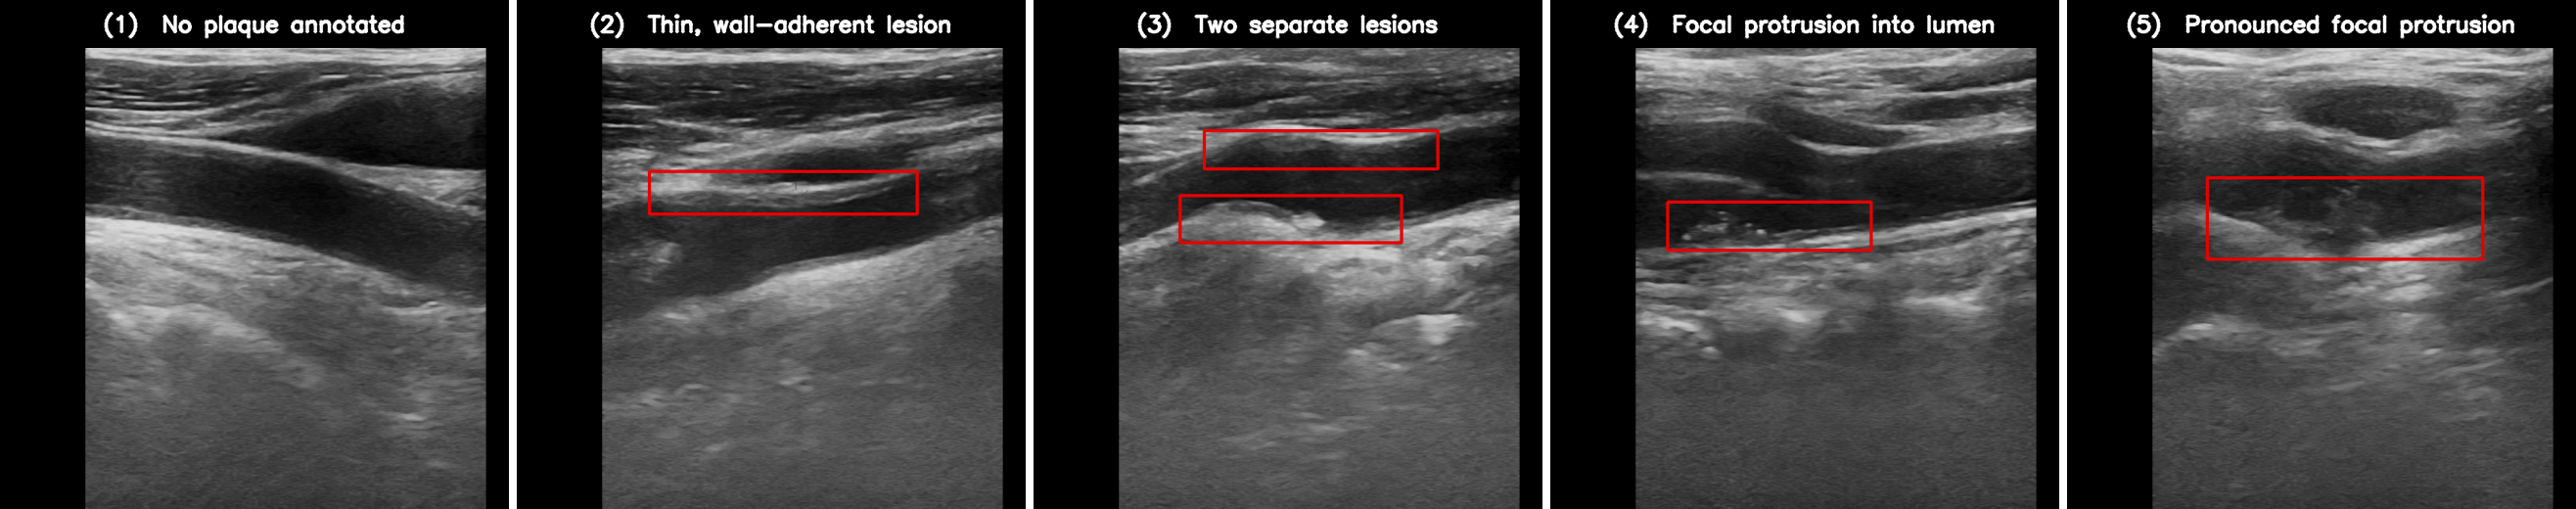
\includegraphics[width=\textwidth]{figures/plaque_progression.png}
\caption[Progression of an atherosclerotic lesion]{Lesion development and its ultrasound
appearance. Carotid artery at five stages of atherosclerotic change --
(1) unaffected vessel wall, (2) initial lipid deposition, (3) early atheroma, (4) fibroatheroma
with a lipid core beneath a fibrous cap, and (5) a complicated lesion with calcification and a
markedly narrowed lumen -- in a B-mode image from Ar-PlaqSegm1
\cite{rulloni2025arplaqsegm1} and an illustration generated with a generative image model
(OpenAI GPT-5.6 Sol, high reasoning effort). The illustration is schematic and carries no
measurement; the prompt used to produce it is archived with the code.}
\label{fig:plaque_progression}
\end{figure}

This sequence is summarised in Figure~\ref{fig:plaque_progression}. Two transitions in it matter
for what follows: the point at which wall thickening becomes a focal protrusion, which is where
the diagnostic criterion applies, and the point at which a lipid-rich core forms, which governs
how the lesion appears in ultrasound.

Clinically, the relevance of a plaque is determined less by the degree of
stenosis it causes than by its propensity to rupture \cite{naghavi2003vulnerable}.
Lesions with a large necrotic core, a thin fibrous cap and intraplaque haemorrhage
are prone to rupture and subsequent thrombus formation, whereas heavily fibrotic or
calcified lesions are comparatively stable; this morphological distinction was
established in coronary arteries \cite{virmani2000lessons} and underlies the
characterisation of carotid lesions as well \cite{libby2021}.

It matters for imaging because the same composition that governs rupture risk also
governs acoustic behaviour: lipid-rich or haemorrhagic tissue appears echolucent
(hypoechoic) in B-mode ultrasound, while fibrous and calcified tissue appears
echogenic (hyperechoic). Figure~\ref{fig:echogenicity} shows both cases. The plaques
that are hardest to delineate against surrounding tissue are therefore, in part, the same ones
that carry the greatest clinical risk. Echolucent plaques are more common in symptomatic than
in asymptomatic patients \cite{plonski2024gsm}, and plaque echogenicity predicts future
vascular events prospectively \cite{tadokoro2014echogenicity}.

The carotid arteries are of particular interest in this context. They are
superficial and therefore accessible to non-invasive ultrasound examination, and
carotid plaque burden is regarded as a marker of systemic atherosclerosis rather
than a purely local finding: subclinical disease is typically present in several
vascular territories at once \cite{fernandezfriera2015pesa}, and carotid involvement
tracks coronary calcification \cite{laclaustra2016femoral}. Carotid plaque presence has been shown to carry
predictive value for future cardiovascular events beyond that of established
risk factors, and to outperform carotid intima-media thickness in this respect. A meta-analysis
of eleven population-based studies covering 54{,}336 participants found plaque the better
predictor of future myocardial infarction, with an area under the curve of 0.64 against 0.61 for
intima-media thickness and a relative diagnostic odds ratio of 1.35 (95\,\% CI 1.10--1.82,
$p = 0.04$) \cite{inaba2012carotid}; a pooled analysis of individual participant data reached the
same conclusion for intima-media thickness as an addition to established risk scores
\cite{denruijter2012cimt}. The margin is real but modest, which is worth keeping in view: the
ten-year infarction rate after a negative finding was 4.0\,\% for plaque against 4.7\,\% for
intima-media thickness. Standardised criteria for assessing carotid
plaque by ultrasound have been set out twice: by the Mannheim consensus, an expert panel
convened at the European Stroke Conferences \cite{touboul2012mannheim}, and in the
recommendations of the American Society of Echocardiography
\cite{johri2020recommendations}.

Assessing plaque burden at the scale of a population cohort, however, is
constrained by the assessment itself. Carotid ultrasound is operator-dependent,
image quality varies with the acquisition protocol and the device used, and
manual plaque annotation requires trained readers and scales poorly: of the
177{,}757 carotid ultrasound images available in the cohort underlying this
thesis, \textcite{omarov2024deep} annotated 680. Automated, image-based
plaque detection is therefore an attractive route to deriving individual-level
plaque phenotypes for large cohorts -- provided such a model transfers reliably
to data other than that on which it was developed, which is the question this
thesis addresses.

\section{Carotid B-Mode Ultrasound}
\label{sec:ultrasound}

B-mode ultrasound forms an image from the echoes of a transmitted pulse. Sound reflects wherever
acoustic impedance changes, and the brightness assigned to a point in the image encodes the
amplitude of the echo returned from that depth \cite{bakhru2013ultrasound}. Boundaries between
tissues of differing density and stiffness therefore appear bright, and homogeneous tissue
appears as a mid-grey texture.

The carotid artery is well suited to this. It lies a few centimetres below the skin, so a
high-frequency probe can be used and resolution is correspondingly fine, and the vessel runs
close to parallel with the skin surface, so a longitudinal section shows a length of wall rather
than a single cross-section. Blood returns almost no echo and the lumen is consequently dark,
while the vessel wall produces the double-line pattern on which the intima-media thickness is
measured: a bright lumen-intima interface, a darker media, and a bright media-adventitia
interface. A plaque appears as material protruding from the wall into that dark lumen, which is
what makes it visible at all.

What it looks like depends on what it is made of. Lipid and intraplaque haemorrhage have acoustic
properties close to those of blood and return little signal, so lipid-rich lesions appear
echolucent and can be difficult to distinguish from the lumen. Fibrous tissue and calcium reflect
strongly and appear echogenic; dense calcification reflects almost the entire pulse and casts an
acoustic shadow, obscuring whatever lies behind it. Figure~\ref{fig:echogenicity} shows the two
extremes of this range in the dataset used here. Because the appearance is graded rather than
categorical, it is often quantified as the grey-scale median of the lesion after normalising the
image against reference structures, which makes values comparable between examinations
\cite{plonski2024gsm}.

Three properties of the modality bear directly on what an automated model can and cannot do with
these images. The first is speckle. The granular texture filling apparently homogeneous tissue is
not structure but interference between echoes from scatterers too small to resolve individually.
It is deterministic for a fixed geometry and changes with any shift of the probe, so it is
reproducible within an image and not between images, and a model may learn from it without the
pattern corresponding to anything anatomical.

The second is that image formation depends on choices made during the examination. Transmit
frequency, depth, focal position, overall gain and depth-dependent gain compensation all alter the
grey levels an identical structure produces, and the angle at which the probe is held alters
whether an interface reflects towards the transducer at all: a wall imaged obliquely returns a
weaker echo than the same wall imaged perpendicularly \cite{bakhru2013ultrasound}. These settings
are chosen by the operator during acquisition and cannot be recovered afterwards from the stored
image.

The third follows from the first two. A B-mode image is not a measurement of tissue in the sense
that a computed tomography number is; it is a record of how a particular vessel appeared to a
particular operator using a particular device at a particular setting. Two examinations of the
same artery may differ visibly without either being wrong. This is the source of the
operator dependence noted above, it is why plaque assessment is reported with agreement
statistics rather than as a measurement error (Section~\ref{sec:plaque-definition}), and it is
the mechanism behind the distribution shift discussed in Section~\ref{sec:domain-shift}.

\begin{figure}[H]
\centering
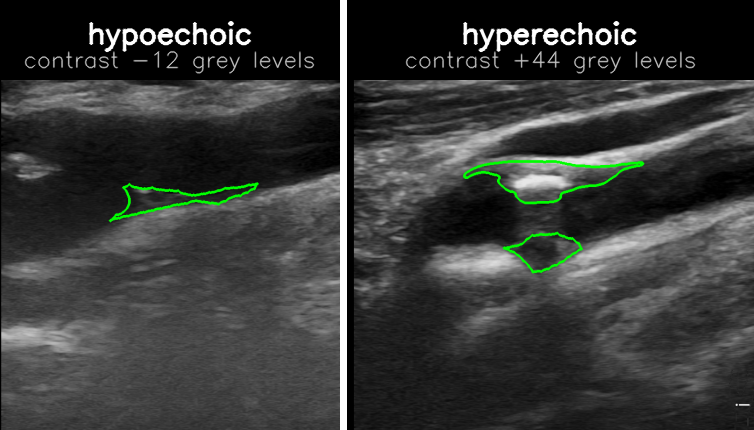
\includegraphics[width=0.82\textwidth]{figures/echogenicity.png}
\caption[Hypoechoic and hyperechoic plaque]{Two annotated images from Ar-PlaqSegm1
\cite{rulloni2025arplaqsegm1} illustrating the range of plaque echogenicity, with the annotation
outlined in green. Left: a hypoechoic lesion, 12 grey levels darker than the tissue immediately
surrounding it. Right: hyperechoic plaque, 44 grey levels brighter. The two examples have almost
the same aspect ratio, 3.9 and 4.3, so the comparison varies echogenicity while holding lesion
shape roughly constant; shape is treated separately in Figure~\ref{fig:focal-vs-diffuse}.
Contrast is the difference in mean intensity between the annotated region and a ring of 25 pixels
around it, excluding any other annotated tissue.}
\label{fig:echogenicity}
\end{figure}

\section{Plaque Definition and Annotation}
\label{sec:plaque-definition}

\begin{figure}[H]
\centering
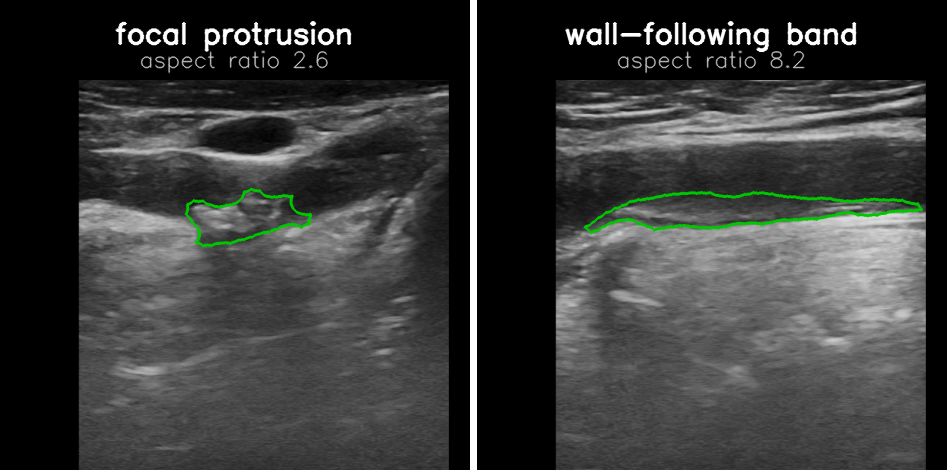
\includegraphics[width=0.82\textwidth]{figures/focal_vs_diffuse.png}
\caption[Focal and elongated annotations]{Two annotated lesions spanning the range of shapes the
plaque criterion has to accommodate, outlined in green. Left: a compact focal protrusion with an
aspect ratio of 2.6. Right: a thin band following the vessel wall over 575 pixels, aspect ratio
8.2. The criterion distinguishes focal protrusion from diffuse wall thickening, and the
boundary between them is where both the annotation and the models are least certain
(Section~\ref{subsec:results-error-analysis}).}
\label{fig:focal-vs-diffuse}
\end{figure}

The criterion this thesis works with is the one set out by the Mannheim consensus, under which a
plaque is ``a focal structure that encroaches into the arterial lumen of at least 0.5\,mm or
50\,\% of the surrounding IMT value or demonstrates a thickness $>1.5$\,mm as measured from the
media-adventitia interface to the intima-lumen interface'' \cite{touboul2012mannheim}. Two of its
three limbs are absolute and one is not, and the difference matters for everything that follows.

The absolute limbs can in principle be evaluated from the lesion alone: a thickness measurement
against a fixed threshold. The relative limb cannot. Whether a given thickening qualifies depends
on the intima-media thickness of the wall on either side of it, so the same structure is a plaque
in a vessel with a thin wall and is not one in a vessel that is uniformly thickened. The
criterion is, in this limb, a comparison rather than a property, and it is the limb that
distinguishes focal disease from diffuse wall thickening. Figure~\ref{fig:focal-vs-diffuse}
contrasts the two extremes of shape that this has to accommodate.

This has a direct consequence for an automated model. A detector or a segmentation network scores
each candidate region on its own appearance; the surrounding wall enters only in so far as it
happens to fall within the receptive field, and the model is never told that the comparison is
what defines the class. Whether it infers the comparison from examples is an empirical question
rather than a design guarantee, and Section~\ref{subsec:results-error-analysis} shows what
happens when it does not: the errors both models share are thickened wall without focal
protrusion, which is precisely the case the relative limb exists to exclude.

Applying the criterion is also not free of judgement when a human does it. Inter-sonographer
agreement for plaque detection under the Mannheim consensus has been reported at
$\kappa = 0.70$ (95\,\% CI 0.60--0.80), which is substantial but not near-perfect, and the
disagreements are systematic rather than random: lesions found in only one of two examinations
were smaller than those found in both, with a mean area of 6.82\,mm$^2$ against 11.65\,mm$^2$ and
a mean thickness of 1.45\,mm against 1.96\,mm \cite{nyman2020reproducibility}. Small plaques near
the threshold are where readers disagree with one another, and Chapter~\ref{ch:results} finds
them to be where the models fail as well.

Two implications for this thesis follow. The annotations a model is trained on are expert
judgements rather than ground truth in the physical sense, so the agreement between two readers
bounds what any model evaluated against a single reader can be expected to achieve. And because
the disagreement concentrates at the small end of the size distribution, an evaluation set with
few small lesions will overstate performance relative to one with many --- which is one reason the
composition of an external dataset, and not only its size, determines what a validation on it
means.
\section{Computational Approaches to Subclinical Atherosclerosis}
\label{sec:automated-detection}

Three kinds of data are routinely used to characterise subclinical atherosclerosis at scale:
images of the vessel, clinical and health-record variables describing the patient, and molecular
measurements from blood. Each has an established computational literature, and the three differ
in what they can resolve.

\subsection{Detection and Segmentation in Carotid Ultrasound}

The bottleneck in assessing carotid plaque across a cohort is image reading rather than image
acquisition. Of the 177{,}757 carotid ultrasound images available in the cohort underlying this
thesis, \textcite{omarov2024deep} annotated 680 -- fewer than 0.4\,\% -- because plaque annotation
requires a trained reader and per-image judgement. Automating that judgement is therefore the
prerequisite for using such images as a source of phenotypes.

Deep learning has made this tractable. Object detection frameworks such as YOLO locate
structures of interest by regressing bounding boxes with an associated confidence score
\cite{redmon2016yolo}, while segmentation architectures such as U-Net delineate them pixel by
pixel \cite{ronneberger2015unet}. In both cases transfer learning allows a model pre-trained on
natural images to be adapted to a specialised domain from a comparatively small annotated set
\cite{shin2016transfer}.
Applied to carotid ultrasound, the approach has been pursued for plaque segmentation
\cite{jain2021hybrid}, for plaque characterisation and classification
\cite{singh2024plaque}, and in a body of work surveyed by \textcite{huang2023review}.

Two features of this literature bear on the present work. The cohorts are typically clinical
rather than population-based: as \textcite{omarov2024deep} note, earlier studies have largely
addressed patients presenting with stroke or individuals with known carotid disease, which limits
how far the resulting models generalise to asymptomatic populations. And the models are
developed and evaluated within a single data source. \textcite{omarov2024deep} is the first
application at population scale, on 19{,}499 UK Biobank participants, and remains evaluated
within that cohort.

\subsection{Risk Estimation from Clinical and Health-Record Data}

An independent tradition estimates cardiovascular risk from patient characteristics rather than
from images. SCORE2 and its counterpart for older adults derive ten-year risk of a first
cardiovascular event from age, sex, smoking status, blood pressure and lipid measurements
\cite{score22021, score2op2021}. The Framingham risk profile \cite{dagostino2008framingham}
and the Pooled Cohort Equations of the American College of Cardiology and the American Heart
Association \cite{goff2014pooled} follow the same principle and are in equally wide clinical
use.

Deep learning has been applied to the same kind of data in a less constrained form. Rather than
combining a fixed set of risk factors, these models read the sequence of coded diagnoses,
medications and measurements in a health record directly \cite{rajkomar2018scalable}, and
transformer architectures developed for language have been adapted to that sequence
\cite{li2020behrt}. The most recent of them, Delphi-2M, was trained on UK Biobank records and
predicts the rates of more than a thousand diseases over the following decades
\cite{shmatko2025delphi}.

What none of these instruments do, however classical or however learnt, is observe the arterial
wall. They estimate risk from its determinants and its consequences, and consequently do not
capture subclinical disease already present in an individual whose recorded profile appears
unremarkable -- which is the gap imaging is expected to fill.

\subsection{Molecular Markers}

A third line of work seeks markers of atherosclerosis in molecules rather than in images, and it
divides by what is measured and at what cost.

At one extreme, proteomic profiling of excised plaque tissue resolves the lesion directly.
\textcite{sinha2026proteomics} analysed 112 carotid endarterectomy specimens and found that the
molecular differences between thin-capped and thick-capped plaques are spatially confined to the
necrotic core and the fibrous cap, enriched for inflammation, lipid handling and matrix
remodelling. Measurements of this kind have the highest fidelity available, because the tissue
itself is analysed, but they require the plaque to have been surgically removed. They are
therefore restricted to patients who proceed to endarterectomy, which excludes the asymptomatic
population in which subclinical atherosclerosis is defined. Notably, the same study derived a
serum protein panel predictive of plaque vulnerability, which indicates that properties of the
lesion can register in circulation.

At the other, plasma proteomic panels are now available for entire cohorts: 2{,}923 proteins have
been measured in some 53{,}000 UK Biobank participants \cite{sun2023plasma}, with comparisons
across measurement platforms established separately \cite{eldjarn2023plasma}. A blood draw
scales in a way that imaging and surgery do not, and it is non-invasive. What it observes,
however, is a systemic state, whose relation to a focal arterial lesion is not fixed by the
measurement itself but has to be established.

Between the two sits the question this thesis begins from: whether circulating proteins reflect a
lesion that has been located by imaging rather than removed by surgery. Answering it requires
both modalities in the same individuals and at a scale at which associations can be detected --
which is possible only if the lesion can be identified automatically.

\subsection{What Is Missing}

Each strand is limited in a different way, and the limitations are complementary rather than
redundant. Imaging observes the disease directly but at a cost that constrains cohort size, and
the models that automate it are rarely shown to transfer between data sources: external
validation remains the exception in medical imaging \cite{kim2019design, varoquaux2022failures}. Risk scores
scale effortlessly but infer rather than observe. Molecular panels scale and observe, but what
they observe is a systemic state whose relation to a focal arterial lesion is unestablished.

Combining them requires a phenotype that is both accurate and available at scale, and it is the
production of that phenotype -- rather than any of the three strands in isolation -- that this
thesis is concerned with.

\section{Domain Shift and External Validation}
\label{sec:domain-shift}

A model that performs well on held-out data from the cohort it was developed on may perform
substantially worse on data from elsewhere. This is not a failure of training but a
consequence of the data distribution changing between development and deployment -- commonly
termed dataset or domain shift \cite{castro2020causality}.

Ultrasound is particularly exposed to it. The image is not a direct measurement of tissue
but the result of an interaction between the tissue, the transducer, the machine's signal
processing, and the operator's choices of angle, depth, gain and focus
\cite{bakhru2013ultrasound}. Device vendor and
model, the acquisition protocol in force at a given centre, and the demographic composition
and disease prevalence of the imaged population all shift the distribution a model sees.
A model can absorb any of these as if they were features of the disease.
\begin{figure}[H]
\centering
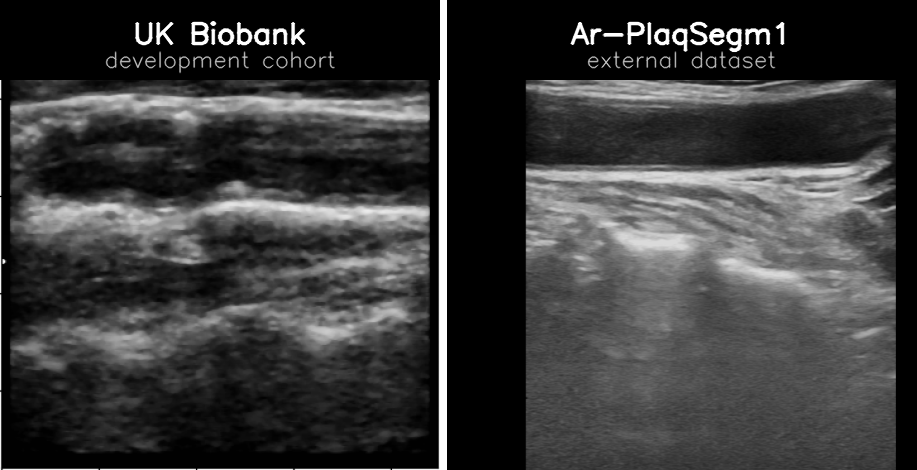
\includegraphics[width=0.86\textwidth]{figures/domain_shift.png}
\caption[Two acquisitions of the same anatomy]{The same anatomical structure recorded in the two
datasets used in this thesis, shown at a common scale. Left: a UK Biobank acquisition, the cohort
on which the base model was developed. Right: an image from Ar-PlaqSegm1
\cite{rulloni2025arplaqsegm1}, the external dataset it is evaluated on in
Chapter~\ref{ch:results}. The two differ in brightness, speckle texture and field of view
although both depict a longitudinal section of the carotid artery. Section~\ref{sec:phase2}
quantifies what such differences cost in model performance.}
\label{fig:domain-shift}
\end{figure}

Figure~\ref{fig:domain-shift} shows what this amounts to in practice for the two datasets used
here.

The effect is documented for ultrasound specifically. A model trained on one scanner loses
accuracy when applied to images from another, and recovers it only once the target device is
accounted for \cite{soylu2025migration}. A lung ultrasound classifier developed at a single
centre retained a sensitivity of 0.92 on multicentre data but fell to a specificity of 0.76,
which fine-tuning on part of that data raised to 0.82 while sensitivity stayed unchanged
\cite{wu2024generalizability} -- a pattern of preserved sensitivity and degraded specificity
that recurs in Chapter~\ref{ch:results}.

Internal validation does not detect this. Cross-validation and a held-out test set drawn
from the same cohort both estimate how a model generalises to unseen \emph{samples} of the
same distribution; neither estimates how it generalises to a different one. Reporting
standards for clinical prediction models and for artificial intelligence in medical imaging
therefore ask explicitly for validation on data external to the development cohort
\cite{collins2015tripod, mongan2020claim}. \textcite{omarov2024deep} report
five-fold cross-validation and a blind test set of 103 images, both drawn from UK Biobank;
performance outside that cohort is, by construction, not addressed by either.

In this thesis the consequence is concrete. The plaque model is not the final result: its
output is the variable that the proteomic and health-record analyses then take as their
exposure. Every participant the model labels incorrectly enters those analyses with the wrong
plaque status. Misclassification of this kind is non-differential -- the model cannot see the
protein measurements, so its errors are unrelated to the outcome -- and non-differential
misclassification biases estimated associations towards the null
\cite{copeland1977bias}. A degraded phenotype therefore weakens precisely the associations
such analyses are looking for, and does so silently, since the analysis itself gives no
indication that the exposure was measured with error. Quantifying the performance gap outside the
development cohort is therefore a prerequisite for interpreting any result derived from the
model, and reducing that gap is the subject of the second part of this thesis.

\section{Aim of This Thesis}
\label{sec:aim}

The aim of this work is to establish whether circulating proteins carry a detectable signature of
subclinical carotid atherosclerosis, and -- where that question meets its limits -- to improve the
means by which the disease is measured in the first place.

Both parts rest on the same prerequisite. Carotid plaque is not recorded as a variable in a
population cohort; it exists only implicitly, in ultrasound images that no one has read. Any
analysis relating plaque to molecular or clinical data must therefore begin by producing the
phenotype, and the quality of everything downstream is bounded by the quality of that production
step. This thesis takes that dependency as its organising principle: it derives the phenotype,
uses it, and then examines the model that produces it.

One constraint shapes the design from the outset. Carotid ultrasound and plasma proteomics were
acquired in different subsets of the cohort: the Olink panel covers 52{,}998 samples and a
plaque phenotype can be derived for 20{,}014 participants, but only 2{,}542 participants belong
to both. Any analysis relating the two directly is confined to that intersection, and the
remaining fifty thousand proteomic profiles cannot contribute, because no imaging exists for
them.

The original objective of this work addressed that constraint rather than accepting it. Health
records, unlike imaging, are available for essentially the whole cohort. If the plaque phenotype
derived from ultrasound could be predicted from health-record variables -- a proxy plaque score,
fitted on the 20{,}014 participants for whom both are available -- then that proxy could be
evaluated for every participant with proteomic data, and the association between atherosclerosis
and the plasma proteome could be tested at twenty times the sample size. The imaging arm would
supply the ground truth; the health records would supply the reach.

Three lines of work follow from this design. The first applies the detection model of
\textcite{omarov2024deep} across the UK Biobank carotid ultrasound collection and relates the
resulting plaque phenotype to the Olink proteomic panel on the intersection of the two, protein
by protein and as a multivariate predictor. The second was to construct the proxy score and
extend the analysis to the full proteomic set; it could not be carried out, as access to the
platform holding the data ended during preparation. The third, which forms the substantive
contribution of this thesis, turns to the detection model itself: how it performs on carotid
ultrasound acquired outside the cohort it was developed on, whether a model formulation matched
to the available annotations improves on it, and what limits the result. The dependency runs in
one direction throughout -- the proxy score would have been fitted against the imaging phenotype,
so its ceiling is set by the quality of that phenotype, which is what the third line of work
addresses.

The specific objectives are:

\begin{enumerate}[nosep]
  \item to reproduce the detection pipeline of \textcite{omarov2024deep} on the full set of
        UK Biobank carotid ultrasound images, and to derive individual-level plaque presence
        and plaque counts from it;
  \item to test whether the resulting plaque phenotype is associated with plasma proteomic
        profiles, both protein by protein and as a multivariate predictor;
  \item to construct a health-record-based proxy for that phenotype, so that the proteomic
        analysis is no longer restricted to the small subset of participants who have both
        imaging and proteomic measurements;
  \item to quantify the performance of that model on an external dataset of B-mode carotid
        ultrasound images, and thereby the magnitude of the distribution shift between its
        development cohort and an independent one;
  \item to fine-tune instance segmentation models on that dataset, which consume the available
        pixel-level annotations directly rather than reducing them to bounding boxes, and to
        evaluate them under a protocol that selects every operating point on validation data
        rather than on the test set; and
  \item to characterise the errors that remain, and to establish which component of the model --
        segmentation quality, instance ranking, or the image-level decision -- constrains its
        performance.
\end{enumerate}

Chapter~\ref{ch:methods} describes the data and the procedures used for each objective,
Chapter~\ref{ch:results} reports the findings, and Chapter~\ref{ch:discussion} places them
against the literature surveyed above.
